
\subsubsection{Exploration Time}
\label{subsubsec:agg-time}

\begin{figure}[h]
\vspace{-8pt}
	\centering
		\subfloat[OpenVX: Diff \#ACCs] {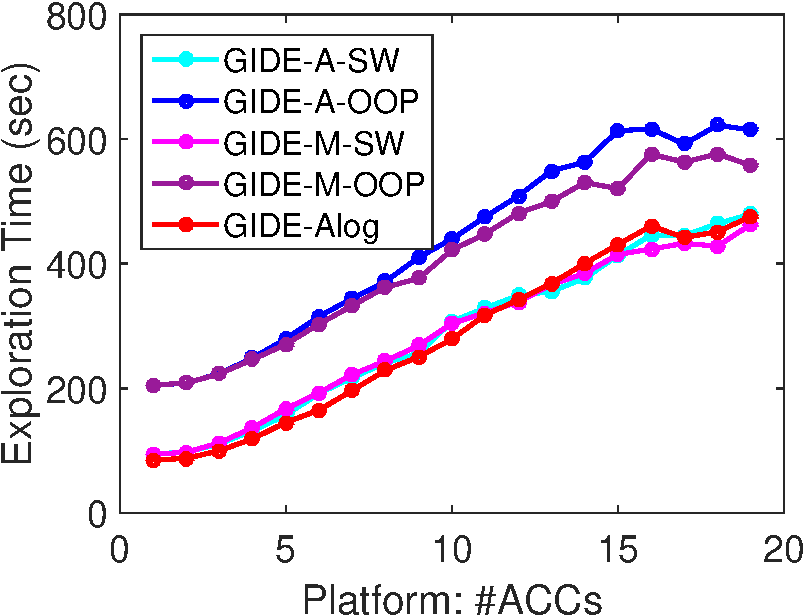
\includegraphics[width=.48\linewidth]{fig/timeACCs.pdf}\label{fig:timeACCs}}
		\hfill
		\subfloat[Synthetic: Diff \#Apps] {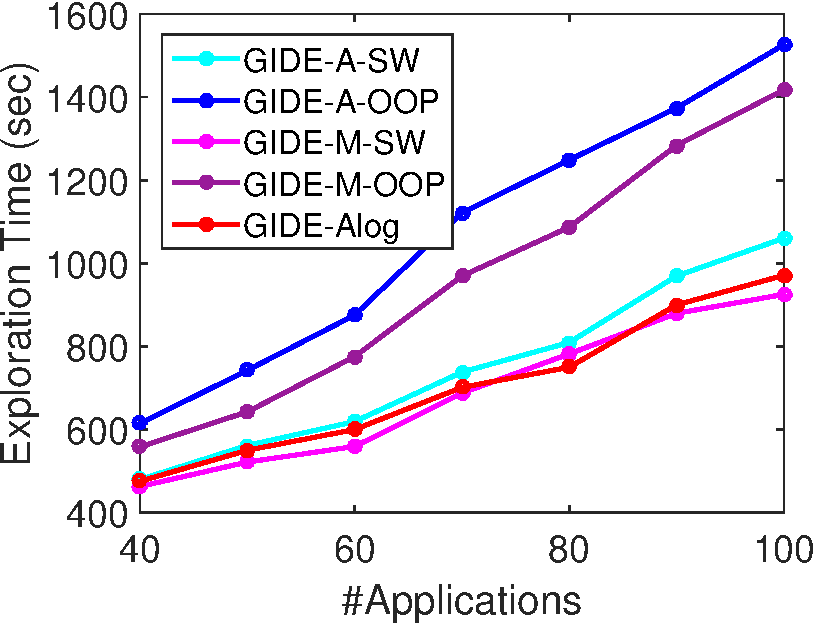
\includegraphics[width=.48\linewidth]{fig/timeApps.pdf}\label{fig:timeApps}}
	\vspace{-8pt}
	\caption{Exploration Time}
	\label{fig:exTime}
\end{figure}

\newtext{
\figref{fig:exTime} shows the exploration time  of MAAR DSE with different aggregations running on Intel i5-3450 with 3.10GHz. In \figref{fig:timeACCs}, the DSE exploration time increases with the increasing of ACCs budget.  
the $A \mhyphen OOP$ and $M \mhyphen OOP$ are much slower than other DSEs, because they need to find the OPT platform of each application for efficiency normalization. In average, the time of finding OPT platforms in $A \mhyphen OOP$ and $M \mhyphen OOP$ takes 32.56\% of total exploration. While, $A \mhyphen SW$, $M \mhyphen SW$ and $Alog$ evaluations do not need these OPT platforms. 
After ACCs>16, DSE exploration time stops increasing, because there is only 35 OpenVX unique kernels in applications, which could be instantiated once in HW. The design complexity of 16-19 ACCs from 35 kernels are not increased significantly.


\figref{fig:timeApps} describes the exploration time with increasing number of applications, which are synthetically generated.
With the number of application increasing, the $A \mhyphen OOP$ and $M \mhyphen OOP$ exploration time increases much faster than $A \mhyphen SW$, $M \mhyphen SW$ and $Alog$. The reason is that the number of application OPT platform search dramatic increases the exploration time of $M \mhyphen OOP$ and $A \mhyphen OOP$. 
}


\begin{table}[h]
	\caption{Comparison of Aggregations in MAAR DSE}
	\vspace{-8pt}
	\label{tab:cmp}
	\centering
	\begin{tabular}{p{0.125\linewidth}|p{0.25\linewidth}|p{0.25\linewidth}|p{0.175\linewidth}}
		\toprule
		& $rEFF_{SW}$ View & $rEFF_{OOP}$ View & Scalability \\
		\midrule
		
		\hline
		A-SW & Bad (low- med- EFF apps) & Bad (low- med- EFF apps) & Good \\
		\hline
		A-OOP & Good & Good & Bad \\
		\hline
		M-SW & Bad (high- EFF apps) & Bad (all apps) & Good \\
		\hline
		M-OOP & Bad (low- med- EFF apps) & Bad (low- EFF apps) & Bad \\
		\hline
		Alog & Good & Good & Good \\
		
		\bottomrule
	\end{tabular}
\end{table}

\newtext{
\tabref{tab:cmp} summaries the performance of MAAR DSE with different aggregations. $A \mhyphen SW$ has a good for scalability, however platform efficiency is bad for low- and med- efficiency applications. $A \mhyphen OOP$ platform achieves high efficient for all applications, but it has a bad scalability, since its normalization needs to explore the OPT platform for each application. Both $M \mhyphen SW$ and $M \mhyphen OOP$ platforms have bad efficiency, because they are only focus on the med- efficiency application in a certain view ($rEFF_{SW}$ or $rEFF_{OOP}$).
We select $Alog$ as aggregation, since it is efficient and fair to all applications. Moreover, it eliminates the need to compute the  normalization, i.e. finding the OPT platform for each application (a DSE problem in itself).
}